\chapter{Appendix C: Annual avarage load profiles} \label{all_load_profile}
%
\begin{figure}[htbp]  
\centering
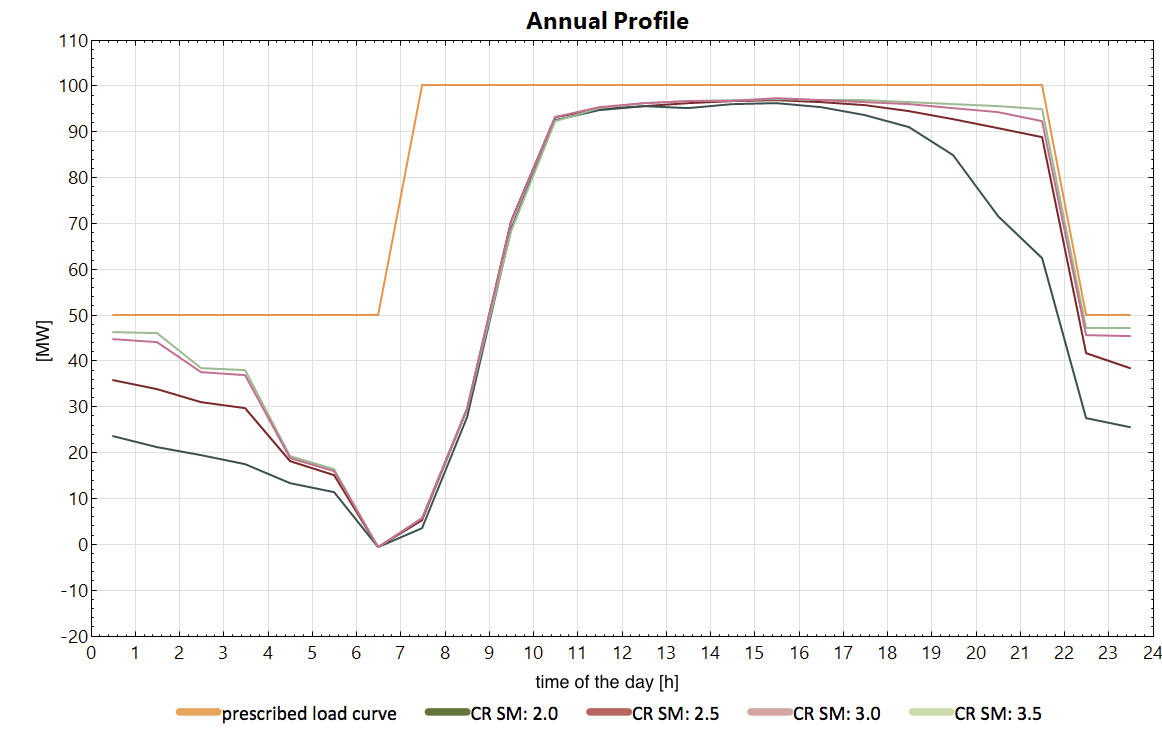
\includegraphics[width=0.8\linewidth]{FIG/Appendix_LCC/CR8h}
\caption[Annual average load profile of CR power plant using 8~h of TES.]{Annual average load profile of CR power plant using 8~h of TES.}\label{CR8h}
\end{figure}
%
\begin{figure}[htbp]  
\centering
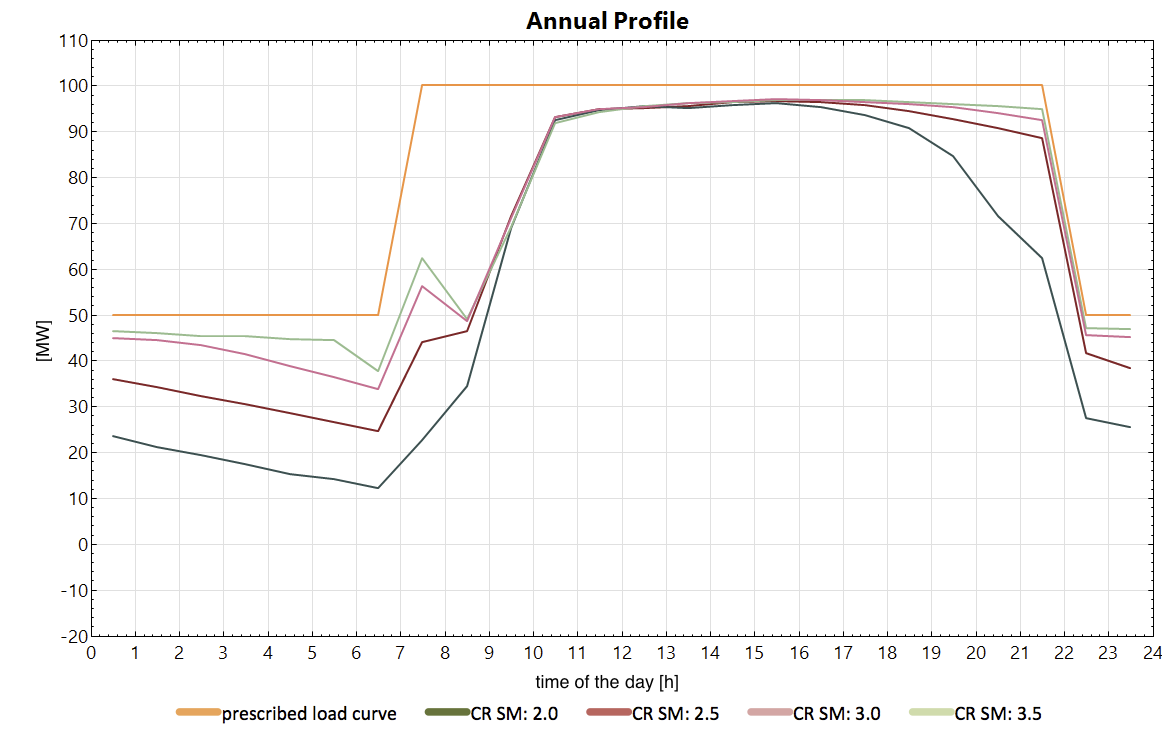
\includegraphics[width=0.8\linewidth]{FIG/Appendix_LCC/CR10h}
\caption[Annual average load profile of CR power plant using 10~h of TES.]{Annual average load profile of CR power plant using 10~h of TES.}\label{CR10h}
\end{figure}
%
\begin{figure}[htbp]  
\centering
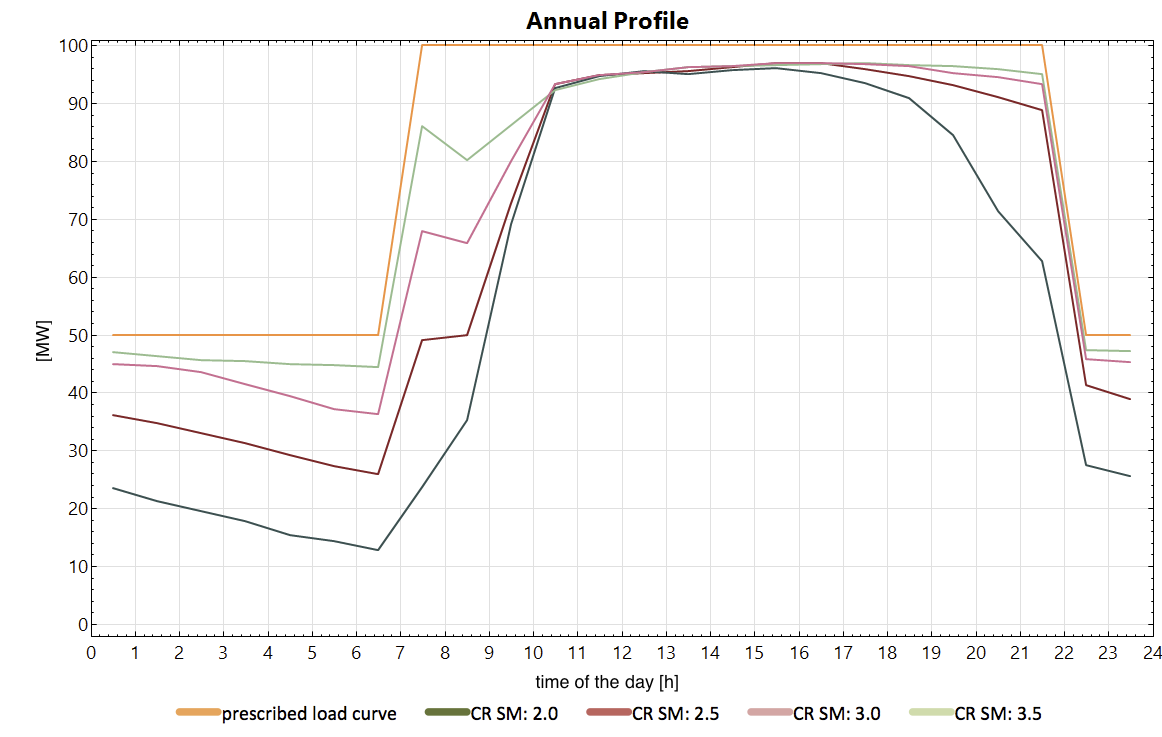
\includegraphics[width=0.8\linewidth]{FIG/Appendix_LCC/CR12h}
\caption[Annual average load profile of CR power plant using 12~h of TES.]{Annual average load profile of CR power plant using 12~h of TES.}\label{CR12h}
\end{figure}
%
\begin{figure}[htbp]  
\centering
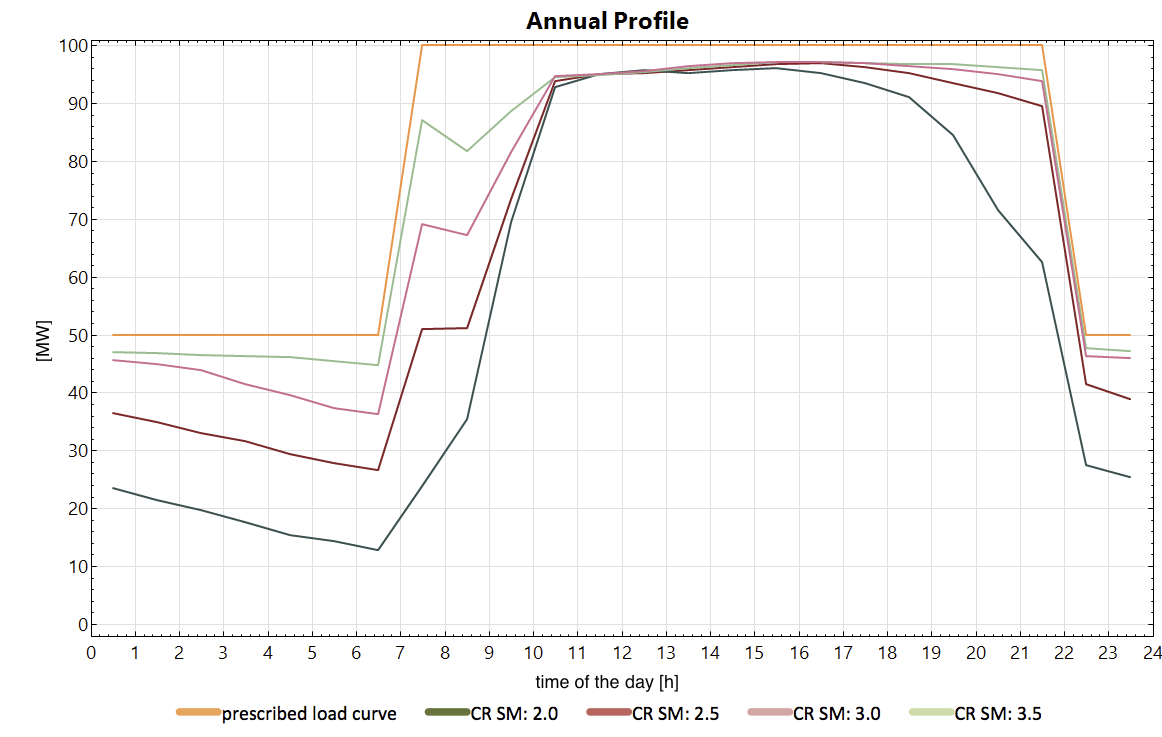
\includegraphics[width=0.8\linewidth]{FIG/Appendix_LCC/CR14h}
\caption[Annual average load profile of CR power plant using 14~h of TES.]{Annual average load profile of CR power plant using 14~h of TES.}\label{CR14h}
\end{figure}
%
\begin{figure}[htbp]  
\centering
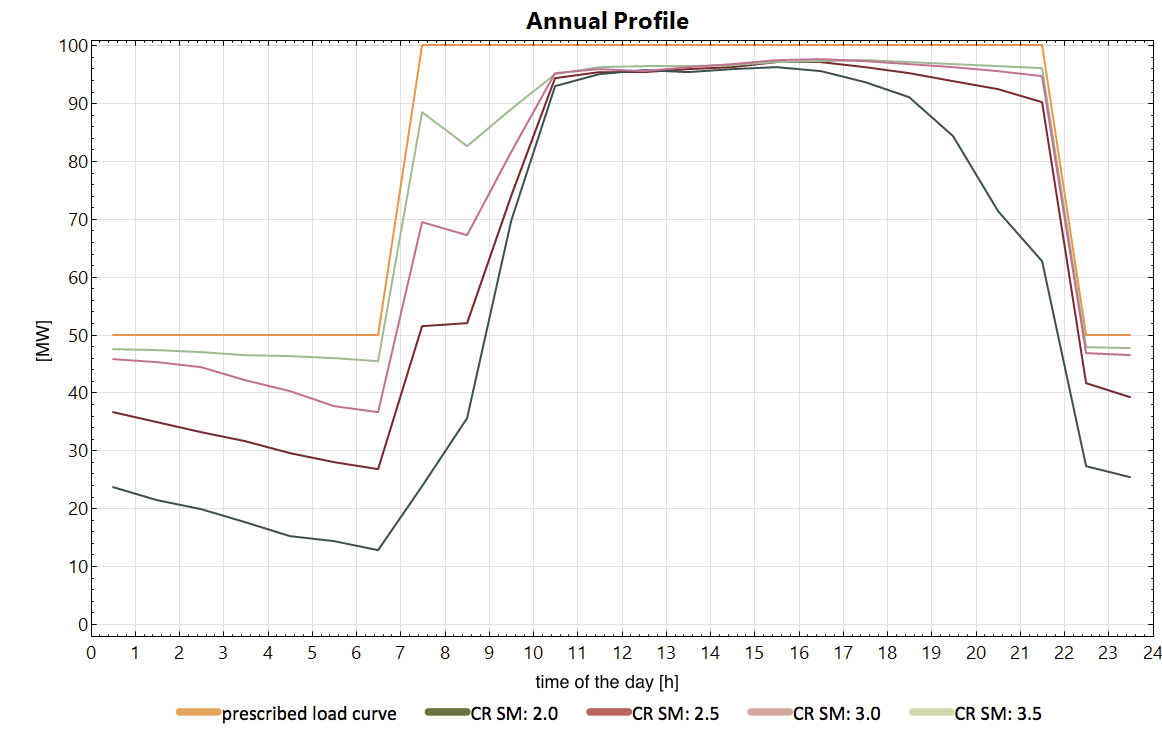
\includegraphics[width=0.8\linewidth]{FIG/Appendix_LCC/CR16h}
\caption[Annual average load profile of CR power plant using 16~h of TES.]{Annual average load profile of CR power plant using 16~h of TES.}\label{CR16h}
\end{figure}
%
\begin{figure}[htbp]  
\centering
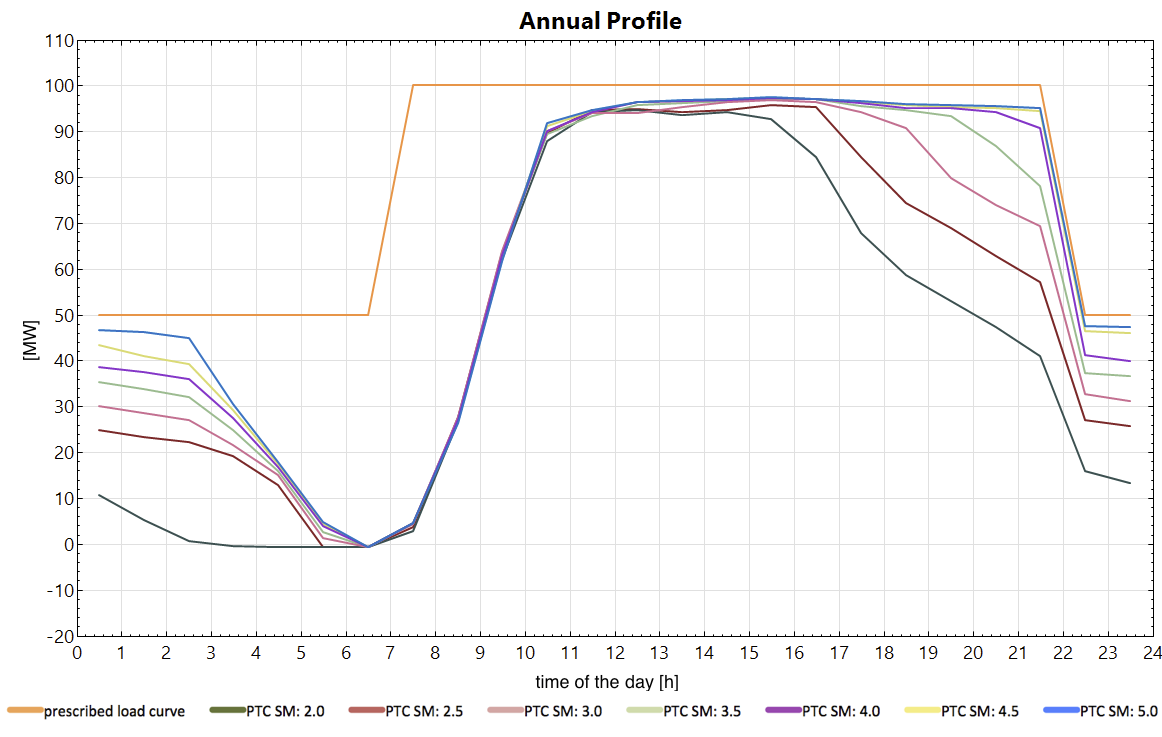
\includegraphics[width=0.8\linewidth]{FIG/Appendix_LCC/PTC8h}
\caption[Annual average load profile of PTC power plant using 8~h of TES.]{Annual average load profile of PTC power plant using 8~h of TES.}\label{PTC8h}
\end{figure}
%
\begin{figure}[htbp]  
\centering
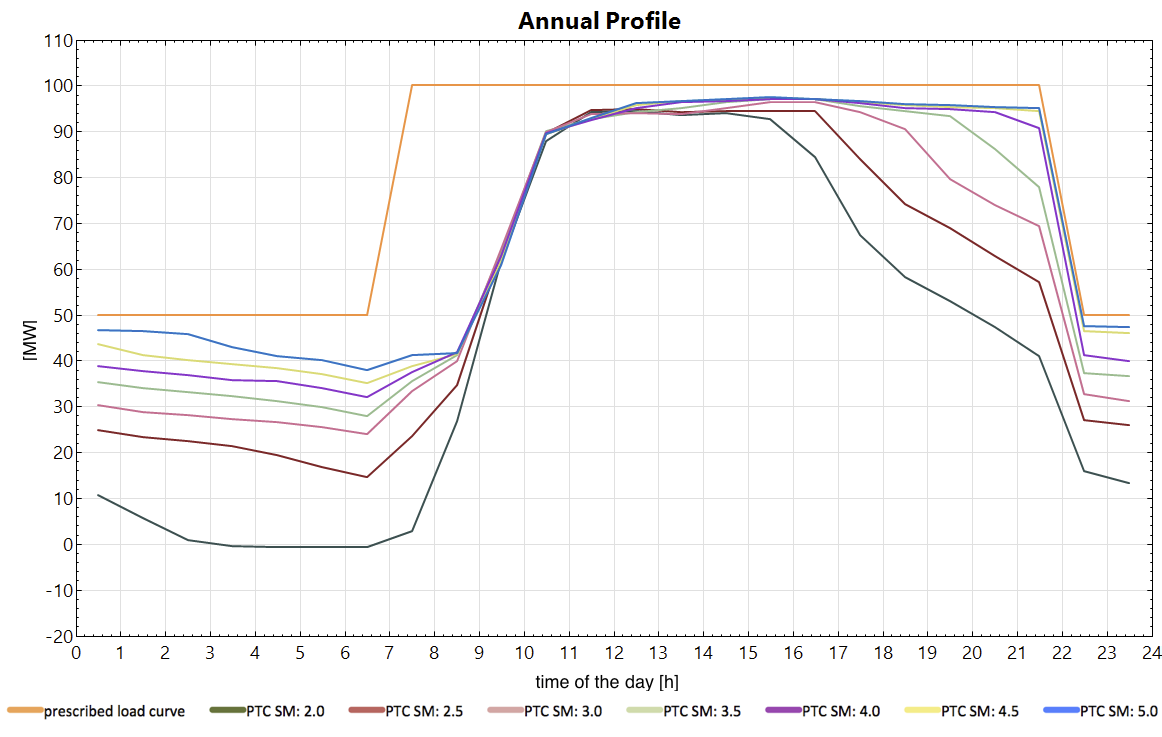
\includegraphics[width=0.8\linewidth]{FIG/Appendix_LCC/PTC10h}
\caption[Annual average load profile of PTC power plant using 10~h of TES.]{Annual average load profile of PTC power plant using 10~h of TES.}\label{PTC10h}
\end{figure}
%
\begin{figure}[htbp]  
\centering
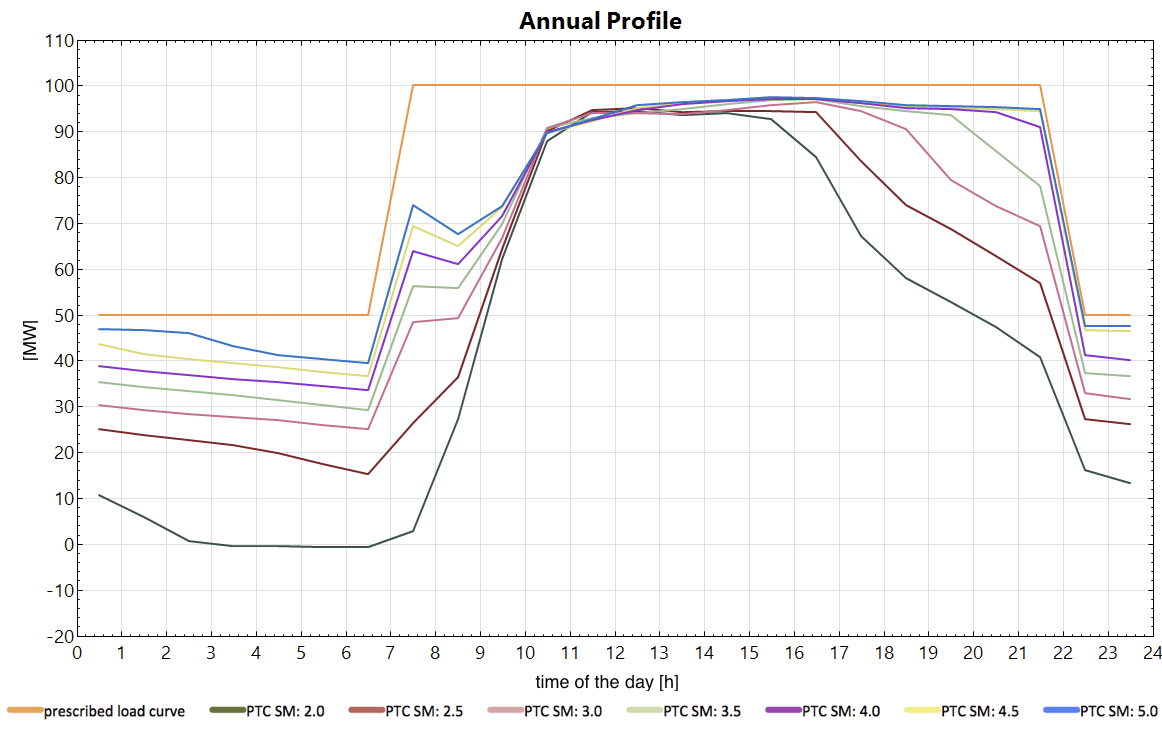
\includegraphics[width=0.8\linewidth]{FIG/Appendix_LCC/PTC12h}
\caption[Annual average load profile of PTC power plant using 12~h of TES.]{Annual average load profile of PTC power plant using 12~h of TES.}\label{PTC12h}
\end{figure}
%
\begin{figure}[htbp]  
\centering
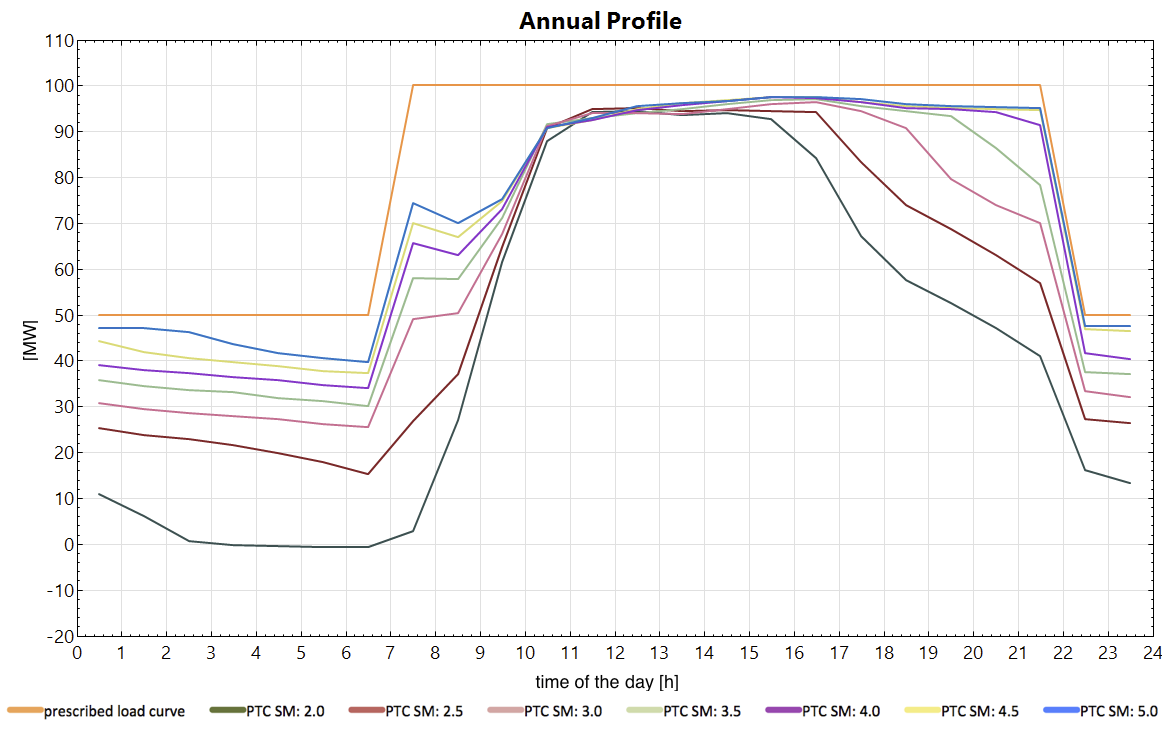
\includegraphics[width=0.8\linewidth]{FIG/Appendix_LCC/PTC14h}
\caption[Annual average load profile of PTC power plant using 14~h of TES.]{Annual average load profile of PTC power plant using 14~h of TES.}\label{CR14h}
\end{figure}
%
\begin{figure}[htbp]  
\centering
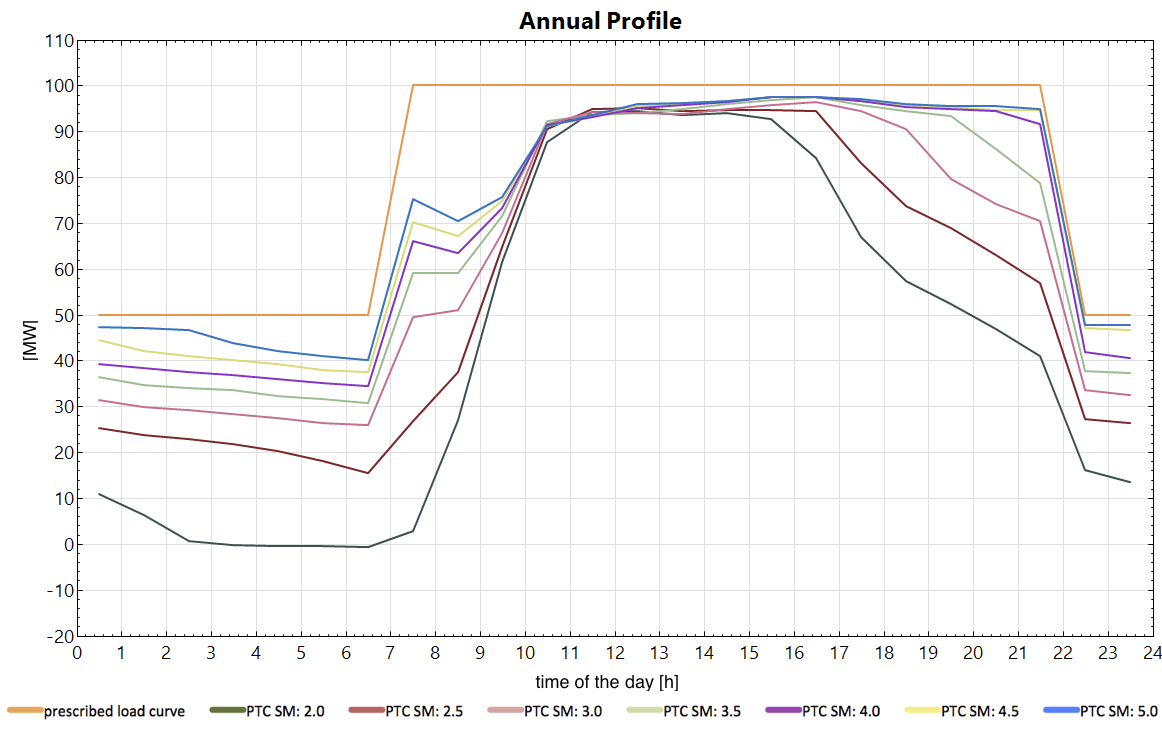
\includegraphics[width=0.8\linewidth]{FIG/Appendix_LCC/PTC16h}
\caption[Annual average load profile of PTC power plant using 16~h of TES.]{Annual average load profile of PTC power plant using 16~h of TES.}\label{PTC16h}
\end{figure}
%
\begin{figure}[htbp]  
\centering
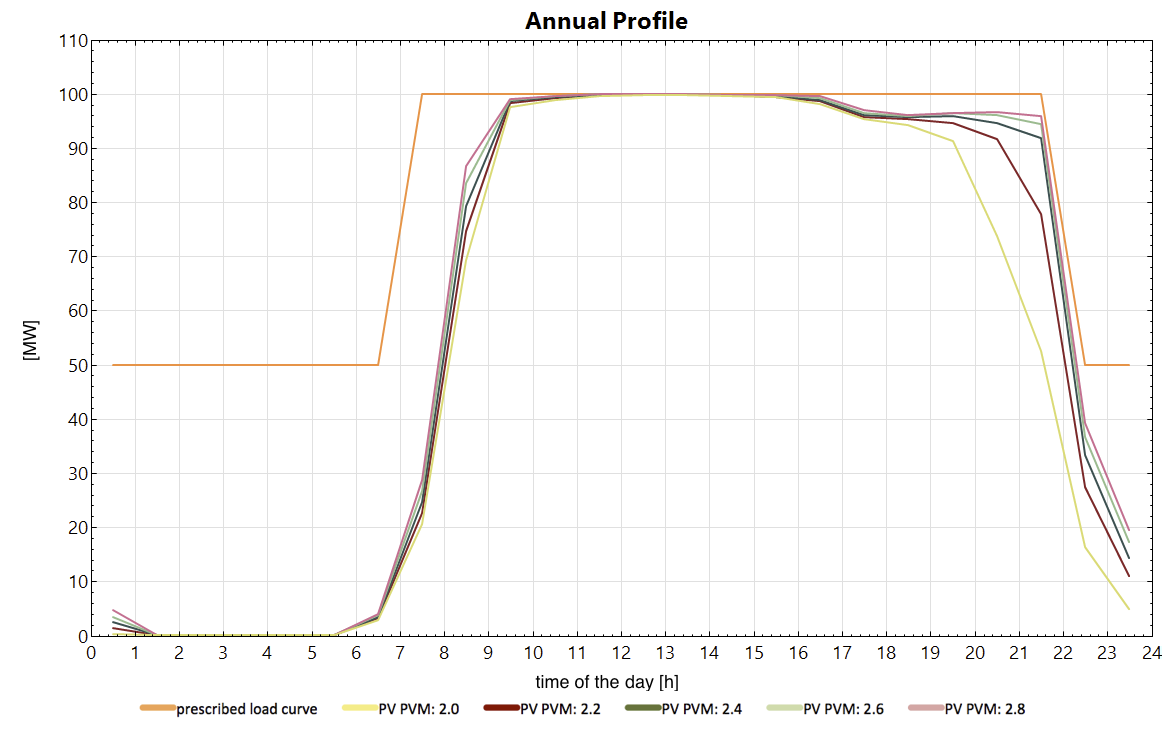
\includegraphics[width=0.8\linewidth]{FIG/Appendix_LCC/PV4h}
\caption[Annual average load profile of PV power plant using 4~h of TES.]{Annual average load profile of PV power plant using 4~h of TES.}\label{PV4h}
\end{figure}
%
\begin{figure}[htbp]  
\centering
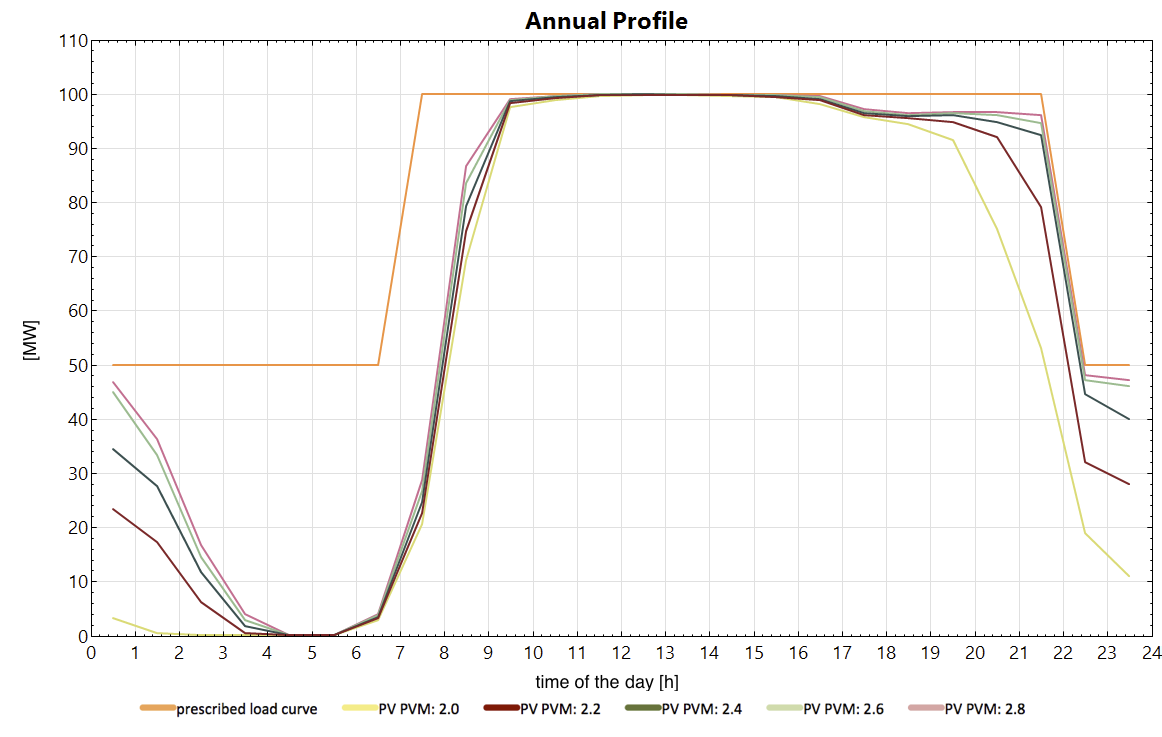
\includegraphics[width=0.8\linewidth]{FIG/Appendix_LCC/PV5h}
\caption[Annual average load profile of PV power plant using 5~h of TES.]{Annual average load profile of PV power plant using 5~h of TES.}\label{PV5h}
\end{figure}
%
\begin{figure}[htbp]  
\centering
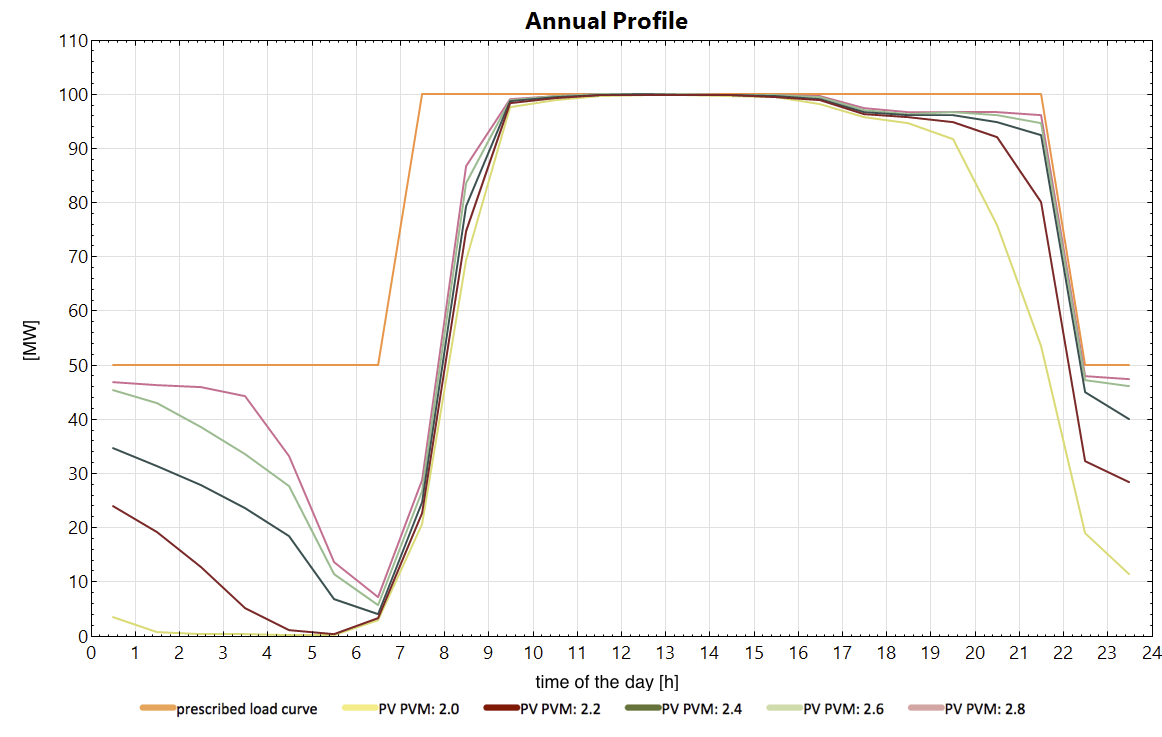
\includegraphics[width=0.8\linewidth]{FIG/Appendix_LCC/PV6h}
\caption[Annual average load profile of PV power plant using 6~h of TES.]{Annual average load profile of PV power plant using 6~h of TES.}\label{PV6h}
\end{figure}
%
\begin{figure}[htbp]  
\centering
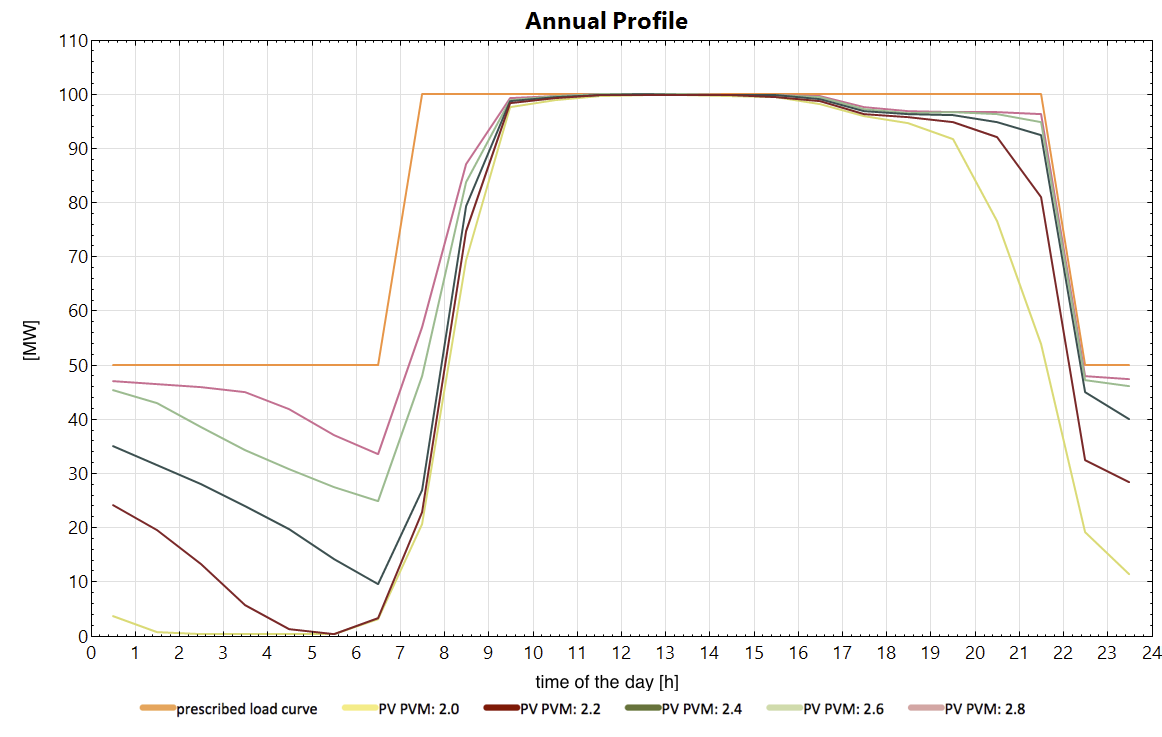
\includegraphics[width=0.8\linewidth]{FIG/Appendix_LCC/PV7h}
\caption[Annual average load profile of PV power plant using 7~h of TES.]{Annual average load profile of PV power plant using 7~h of TES.}\label{PV7h}
\end{figure}
%
\begin{figure}[htbp]  
\centering
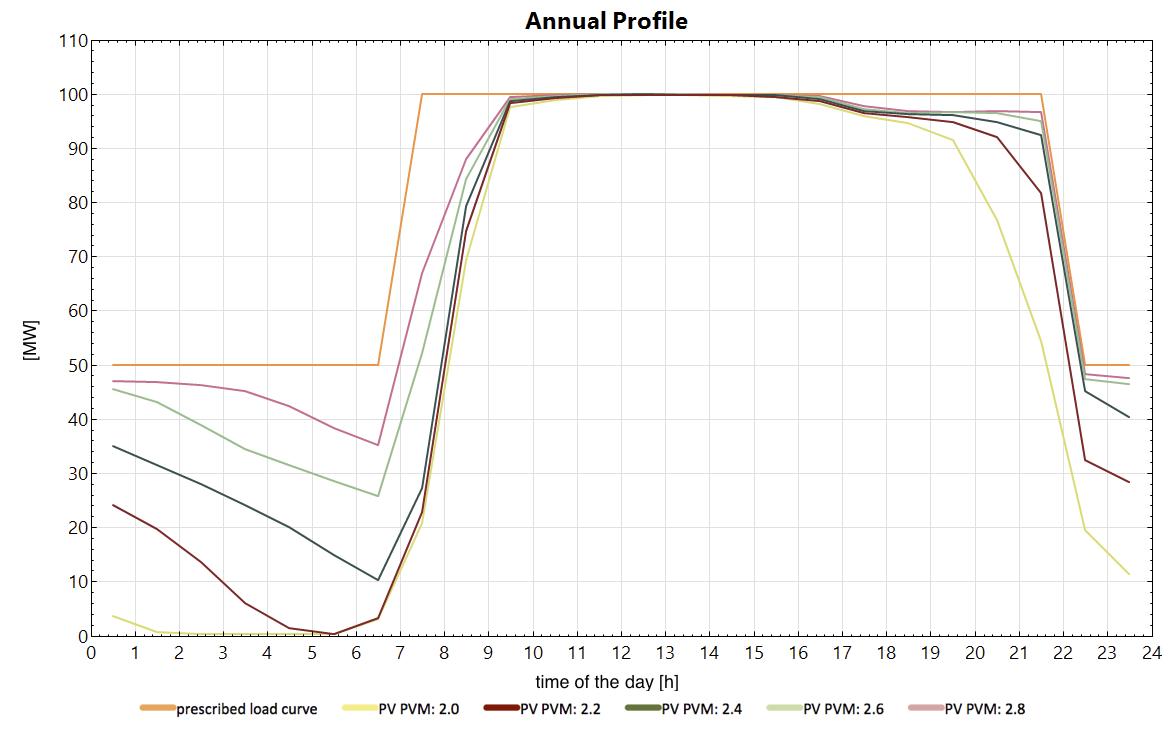
\includegraphics[width=0.8\linewidth]{FIG/Appendix_LCC/PV8h}
\caption[Annual average load profile of PV power plant useing 8~h of TES.]{Annual average load profile of PV power plant useing 8~h of TES.}\label{PV8h}
\end{figure}
%

\pagebreak